\chapter{Lecture 18: Observer and Decorator Patterns, Big Five Revisited}
\begin{center}
\textit{March 13, 2018}
\end{center}

\section{The Observer Pattern}
Last time: the subject publishes, observers subscribe.

\begin{figure}[H]
\centering
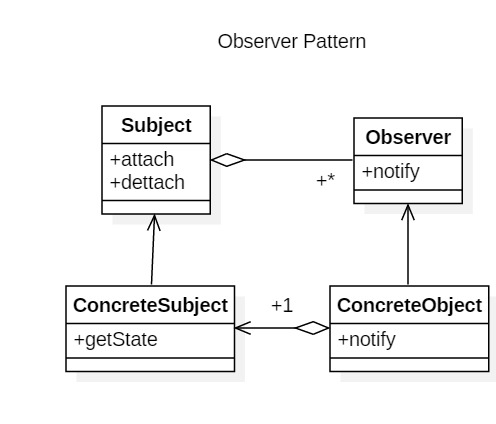
\includegraphics[width=0.6\textwidth]{figures/observer-uml.jpg}
\caption{Observer pattern (UML). A Subject aggregates any number of Observers;
each ConcreteObserver knows its ConcreteSubject so it can call
\code{getState()}.}
\end{figure}

\begin{lstlisting}[style=cpp]
class Observer {
  public:
    virtual void notify() = 0;
    virtual ~Observer() {}
};

class Subject {
    std::vector<Observer*> observers;
  public:
    void attach(Observer *o) { observers.emplace_back(o); }
    void detach(Observer *o) {
        for (auto it = observers.begin(); it != observers.end(); ++it) {
            if (*it == o) { observers.erase(it); break; }
        }
    }
    void notifyObservers() {
        for (auto &o : observers) o->notify();
    }
    virtual ~Subject() = 0;
};
\end{lstlisting}

We want \code{Subject} to be abstract, but it has no obvious pure virtual method
(every subject attaches/detaches/notifies the same way). Trick: make the
\emph{destructor} pure virtual.

\paragraph{Problem.} The dtor of a subclass of \code{Subject} will call the base
class's dtor --- which has no implementation, so the program won't link.

\paragraph{Solution.} Implement \code{Subject}'s dtor anyway:
\begin{lstlisting}[style=cpp]
// subject.cc
Subject::~Subject() {}
\end{lstlisting}
A pure virtual method \emph{may} have an implementation. ``Pure virtual'' means
a subclass must override it to be concrete (for a dtor, every subclass has one
automatically), not that it has no body.

\subsection{Example: A Horse Race}
\begin{lstlisting}[style=cpp]
class HorseRace : public Subject {
    std::ifstream in;          // source of race results
    std::string lastWinner;
  public:
    HorseRace(const std::string &source) : in{source} {}
    bool runRace() { return bool(in >> lastWinner); }
    std::string getState() const { return lastWinner; }
};

class Bettor : public Observer {
    HorseRace *subject;
    std::string name, myHorse;
  public:
    Bettor(HorseRace *hr, const std::string &name, const std::string &horse)
        : subject{hr}, name{name}, myHorse{horse} {
        subject->attach(this);
    }
    ~Bettor() { subject->detach(this); }
    void notify() override {
        std::cout << name
                  << (subject->getState() == myHorse ? " wins!" : " loses.")
                  << std::endl;
    }
};

int main() {
    HorseRace hr{"races.txt"};
    Bettor larry{&hr, "Larry", "RunsLikeACow"};
    Bettor moe{&hr, "Moe", "Molasses"};
    while (hr.runRace()) hr.notifyObservers();
}
\end{lstlisting}
The subject knows nothing about bettors beyond the \code{Observer} interface, so
new kinds of observers can be added without touching \code{HorseRace}.

One round of the race loop, as objects and calls:
\begin{center}
\begin{tikzpicture}[>=Stealth,font=\small,o/.style={draw,rounded corners,fill=green!8,minimum width=2.6cm,minimum height=0.8cm,align=center}]
  \node[draw,rounded corners,fill=blue!6,minimum width=3cm,minimum height=1.2cm,align=center] (hr) at (0,0) {\code{hr}: HorseRace\\ \scriptsize \code{observers} $=$ [\code{\&larry}, \code{\&moe}]};
  \node[o] (l) at (6,1) {\code{larry}: Bettor\\ \scriptsize horse RunsLikeACow};
  \node[o] (m) at (6,-1) {\code{moe}: Bettor\\ \scriptsize horse Molasses};
  \draw[->] ([yshift=4pt]hr.east) -- node[above,sloped,font=\scriptsize]{\code{notify()}} (l.west);
  \draw[->] ([yshift=-4pt]hr.east) -- node[below,sloped,font=\scriptsize]{\code{notify()}} (m.west);
  \draw[->,dashed] (l.north) to[bend right=30] node[above,font=\scriptsize]{\code{subject->getState()}} (hr.north);
  \draw[->,dashed] (m.south) to[bend left=30] node[below,font=\scriptsize]{\code{subject->getState()}} (hr.south);
\end{tikzpicture}
\end{center}

\section{The Decorator Pattern}
We have an object with some behaviour, and while the program is running we want
to add to (enhance) the behaviour of that object. Example: a window, to which we
may add a menu, a scroll bar, a border, \dots{} in any combination.

\begin{figure}[H]
\centering
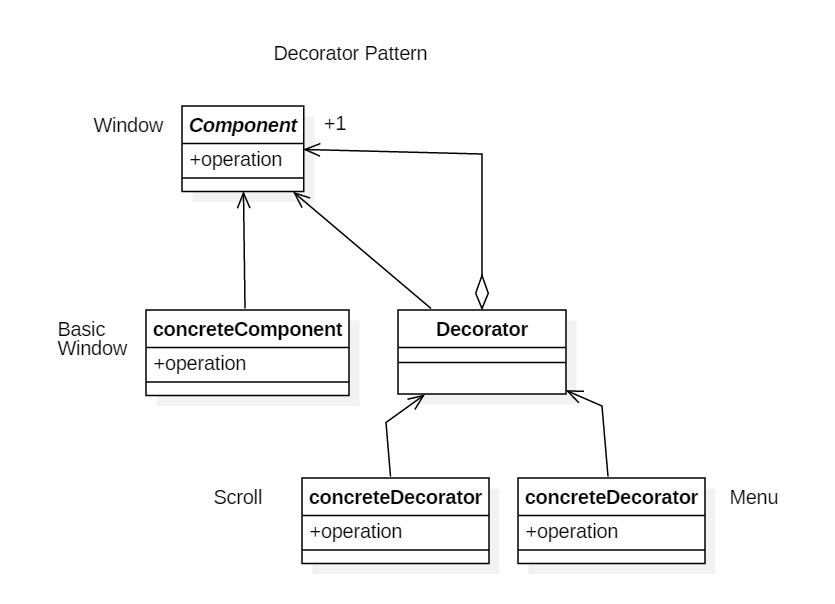
\includegraphics[width=0.75\textwidth]{figures/decorator-uml.jpg}
\caption{Decorator pattern (UML), with the window example: Window is the
abstract component, BasicWindow the concrete component, Scroll and Menu concrete
decorators.}
\end{figure}

\begin{itemize}
  \item \code{Component}: the interface, with the operations to be enhanced.
  \item \code{ConcreteComponent}: the basic object.
  \item \code{Decorator}: an abstract class that \textbf{is-a} Component
        \emph{and} \textbf{has-a} Component (the thing it decorates).
  \item \code{ConcreteDecorator}s: each does its own bit and then delegates to
        the component it wraps.
\end{itemize}
\begin{lstlisting}[style=cpp]
Window *w = new BasicWindow{};
w = new Menu{w};       // a window with a menu
w = new Scroll{w};     // a window with a menu and a scroll bar
w->render();
\end{lstlisting}

\begin{definition}
\textbf{Decorator pattern}: add or enhance behaviour of an existing object at
run time, by wrapping it in objects with the same interface.
\end{definition}

\subsection{Example: Pizza}
\begin{lstlisting}[style=cpp]
class Pizza {                            // Component
  public:
    virtual float price() const = 0;
    virtual std::string desc() const = 0;
    virtual ~Pizza() {}
};

class CrustAndSauce : public Pizza {     // ConcreteComponent
  public:
    float price() const override { return 5.99; }
    std::string desc() const override { return "Pizza"; }
};

class Decorator : public Pizza {         // is-a Pizza
  protected:
    Pizza *component;                    // has-a Pizza
  public:
    Decorator(Pizza *p) : component{p} {}
    virtual ~Decorator() { delete component; }
};

class Topping : public Decorator {
    std::string theTopping;
  public:
    Topping(const std::string &t, Pizza *p) : Decorator{p}, theTopping{t} {}
    float price() const override { return component->price() + 0.75; }
    std::string desc() const override {
        return component->desc() + " with " + theTopping;
    }
};

class StuffedCrust : public Decorator {
  public:
    StuffedCrust(Pizza *p) : Decorator{p} {}
    float price() const override { return component->price() + 2.69; }
    std::string desc() const override {
        return component->desc() + " with stuffed crust";
    }
};

Pizza *p = new CrustAndSauce;
p = new Topping{"cheese", p};
p = new Topping{"mushrooms", p};
p = new StuffedCrust{p};
std::cout << p->desc() << " " << p->price() << std::endl;
// Pizza with cheese with mushrooms with stuffed crust 10.18
delete p;      // deletes the whole chain
\end{lstlisting}
Each decorator owns the component it wraps, so deleting the outermost one frees
everything.

\begin{center}
\begin{tikzpicture}[>=Stealth,font=\small,node distance=0.7cm,
  d/.style={draw,rounded corners,fill=orange!12,minimum height=1cm,align=center,font=\scriptsize},
  c/.style={d,fill=blue!6}]
  \node (p) {\code{p}};
  \node[d,right=0.5cm of p] (s) {StuffedCrust\\ $+2.69$};
  \node[d,right=of s] (m) {Topping\\ mushrooms\\ $+0.75$};
  \node[d,right=of m] (ch) {Topping\\ cheese\\ $+0.75$};
  \node[c,right=of ch] (b) {CrustAndSauce\\ $5.99$};
  \draw[->] (p) -- (s); \draw[->] (s) -- (m);
  \draw[->] (m) -- (ch); \draw[->] (ch) -- (b);
\end{tikzpicture}

\small \code{p->price()} calls inward along the chain and adds on the way back:
$5.99+0.75+0.75+2.69=10.18$.
\end{center}

\section{The Big Five Revisited (with Inheritance)}
\begin{lstlisting}[style=cpp]
class Book {
    ...
  public:
    // defines the Big Five
};
class Text : public Book {
    std::string topic;
  public:
    // does not define the Big Five
};

Text b{"TheFlu", "Nomair", 50, "Medicine"};
Text c = b;     // calls Text's copy ctor
\end{lstlisting}
Remember you get one for free. The free copy ctor of \code{Text} calls Book's
copy ctor on the Book part, then copies the \code{topic} field. Written out, the
free versions are:
\begin{lstlisting}[style=cpp]
// copy ctor
Text::Text(const Text &other) : Book{other}, topic{other.topic} {}

// copy assignment: assign the Book part, then the subclass fields
Text &Text::operator=(const Text &other) {
    Book::operator=(other);
    topic = other.topic;
    return *this;
}
\end{lstlisting}
(\code{Book\{other\}} works because a Text is-a Book: \code{other} binds to
\code{const Book\&}.)

A first (wrong) attempt at the move ctor:
\begin{lstlisting}[style=cpp]
Text::Text(Text &&other) : Book{other}, topic{other.topic} {}   // incorrect
\end{lstlisting}
It won't crash, but it is \emph{copying}, not stealing. (Quick check: if your move
code looks the same as your copy code, it is wrong.)

\begin{aside}
\begin{lstlisting}[style=cpp]
int *p = ...;   // p is a pointer, and p (the variable) is an lvalue
\end{lstlisting}
Likewise, \code{other} has type ``rvalue reference to Text'', but \code{other}
itself is a \emph{named variable}, so it is an \textbf{lvalue}. Hence
\code{Book\{other\}} calls Book's \emph{copy} ctor and \code{topic\{other.topic\}}
calls string's copy ctor.
\end{aside}

We need a way to treat an lvalue as an rvalue: \code{std::move} (from
\code{<utility>}) does exactly that --- it is just a cast to \code{T\&\&}.
\begin{lstlisting}[style=cpp]
Text::Text(Text &&other)
    : Book{std::move(other)}, topic{std::move(other.topic)} {}

Text &Text::operator=(Text &&other) {
    Book::operator=(std::move(other));
    topic = std::move(other.topic);
    return *this;
}
\end{lstlisting}
(Using \code{other.topic} after \code{std::move(other)} is fine: Book's move ctor
only steals the Book part.)

\section{Assignment Through Base Class Pointers}
\begin{lstlisting}[style=cpp]
Text b1{"TheFlu", "Nomair", 50, "Medicine"};
Text b2{"C++IsEasy", "Brad", 500, "CS"};
Book *pb1 = &b1;
Book *pb2 = &b2;
*pb1 = *pb2;     // object assignment through pointers
\end{lstlisting}
\code{Book::operator=} runs (it is non-virtual). Now \code{b1} is
\code{\{"C++IsEasy", "Brad", 500, "Medicine"\}}: only the Book part was assigned.
This is the \textbf{partial assignment problem}.
\begin{center}
\begin{tikzpicture}[>=Stealth,font=\small,f/.style={draw,minimum width=2.4cm,minimum height=0.55cm,font=\scriptsize}]
  \node[font=\scriptsize] at (0,0.55) {\code{b2}};
  \node[f,fill=blue!6] (a1) at (0,0) {C++IsEasy, Brad, 500};
  \node[f,fill=green!10,below=0pt of a1] (a2) {CS};
  \node[font=\scriptsize] at (6,0.55) {\code{b1} afterwards};
  \node[f,fill=blue!6] (b1) at (6,0) {C++IsEasy, Brad, 500};
  \node[f,fill=green!10,below=0pt of b1] (b2) {Medicine};
  \draw[->] (a1) -- node[above,font=\scriptsize]{\code{Book::operator=}} (b1);
  \node[font=\scriptsize,red!60!black,anchor=west] at (b2.east) {\ not copied};
\end{tikzpicture}
\end{center}

\paragraph{Possible solution: make \code{operator=} virtual?}
\begin{lstlisting}[style=cpp]
class Book {
  public:
    virtual Book &operator=(const Book &other);
};
class Text : public Book {
  public:
    Text &operator=(const Text &other) override;  // does not compile:
};                                                // parameter types differ
\end{lstlisting}
To be a valid override, the parameter must be \code{const Book\&}:
\code{Text \&operator=(const Book \&other) override;}. But then \emph{any} Book
can be assigned to a Text: e.g.\ assigning a Comic to a Text through Book
pointers would compile. Not all Books are Texts! This is the \textbf{mixed
assignment problem}.

\paragraph{Alternative: disable assignment through base class pointers.} Make
Book's \code{operator=} non-public:
\begin{itemize}
  \item private? Then subclasses can't call it either (they need it for their
        own \code{operator=}), so it must be \code{protected}.
  \item But Book is not abstract, so then one plain Book could never be assigned
        to another. That says the hierarchy was poorly designed to begin with.
\end{itemize}
The fix (next lecture): an abstract base class with a protected assignment
operator, with plain books as one more concrete subclass.

\section*{Summary}
\begin{itemize}
  \item Observer: Subject keeps a list of \code{Observer*}, notifies them; a pure
        virtual dtor makes a class abstract but still needs a body.
  \item Decorator: is-a and has-a Component; wrap objects to add behaviour at run
        time.
  \item Subclass Big Five must handle the base part (\code{Book\{other\}},
        \code{Book::operator=(other)}).
  \item Inside a move operation the rvalue reference is an lvalue: use
        \code{std::move} to keep moving.
  \item Assigning through base pointers causes partial assignment; a virtual
        \code{operator=} causes mixed assignment.
\end{itemize}
